\documentclass[main]{subfiles}


\begin{document}
\newpage
\section{Reinforcement Learning}
 Reinforcement learning fuses ideas from neuroscience and AI. The model describes how an agent can interact with an environment and in that environment learn to improve its actions when it comes to gathering a targeted reward. 
 
 
  \begin{figure}[H]
	\centering
	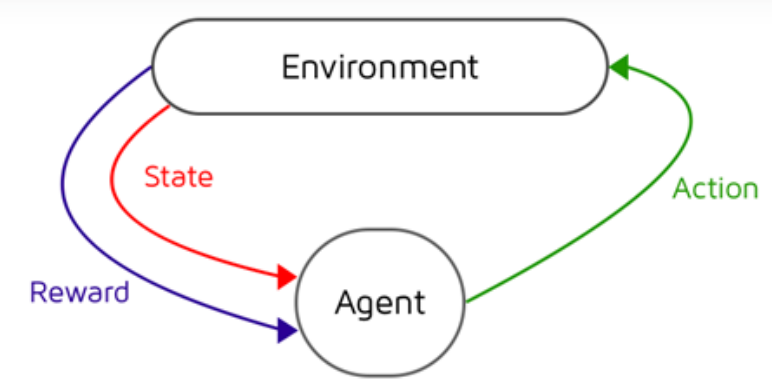
\includegraphics[width=0.9\linewidth]{08_ReinforcementLearning/figures/rl-env-agent-1.png}
	\label{fig:rl-env-agent-1}
	\caption{Connections between an agent and the environment.}
\end{figure}

\begin{itemize}
    \item There is only a reward/supervision signal after each action.
    \item Feedback is often delayed and not instantaneous.
    \item Time needs to be taken into account.
    \item The agent’s actions affect the subsequent data it receives.
\end{itemize}



 \subsection{Dopamine: Reward Prediction Error}
From Schultz (89) \footnote{Predictive Reward Signal of Dopamine Neurons}: Dopamine neurons are activated by rewarding events that are better than predicted, remain uninfluenced by events that are as good as predicted, and are depressed by events that are worse than predicted. Most dopamine nerons show phasic avtivations ... reward-predicting ... However only few phasic activations follow aversive (causing avoidance of a thing) stimuli. By signaling rewards  according to a prediction error, dopamine responses have the formal characteristics of a teaching signal postulated by reinforcement learning theories.
 

  \begin{figure}[H]
	\centering
	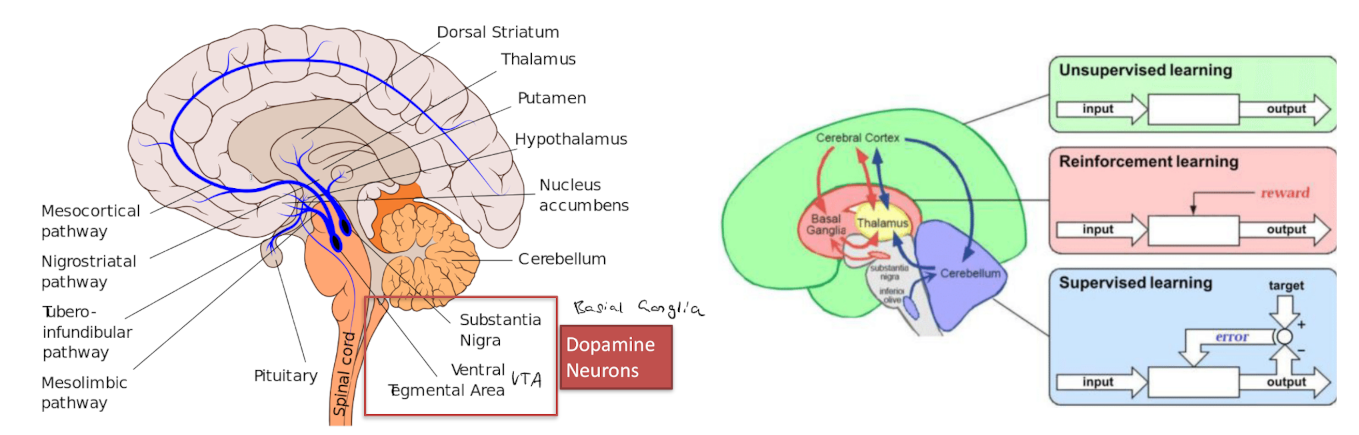
\includegraphics[width=0.9\linewidth]{08_ReinforcementLearning/figures/rl-in-brain.png}
	\label{fig:rl-in-brain}
	\caption{Dopamine neurons of Substantia Nigra and the Ventral Tegmental Area in the Basal Ganglia. (right) Mapping of different machine learning paradigmns to the brain. }
\end{figure}

If the neocortex mostly performs unsupervised learning why does the VTA strongly project to almost all cortical areas and what is the effect of DA on a cortical neuron?

\begin{itemize}
    \item Ventral structure does not project to dorsal (where we assume RL happening).
    \item Gated reinforcement learning: we only want to learn relevant information
    \item Dopamine is connected to plasticity because it is very sensitive to new / unseen data.
\end{itemize}

\begin{figure}[H]
	\centering
	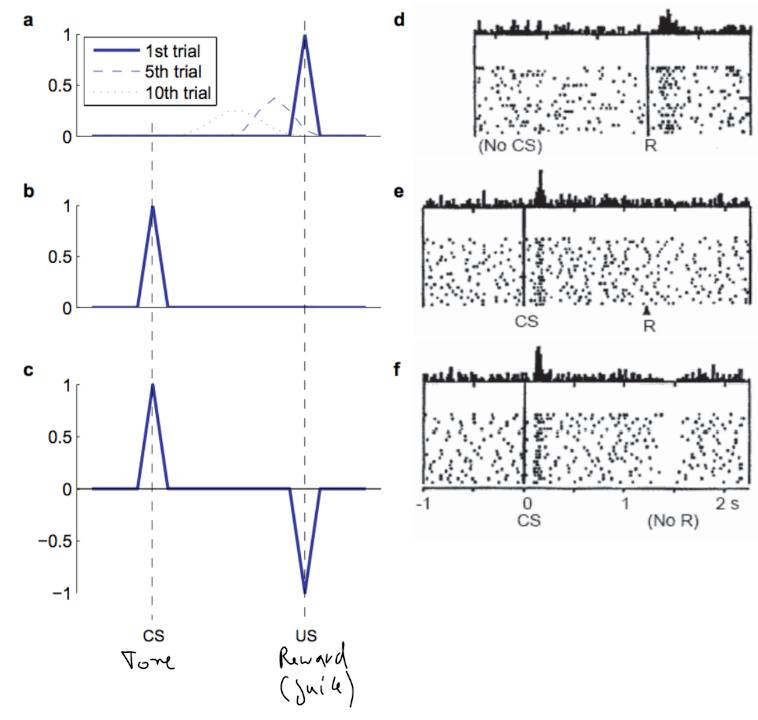
\includegraphics[width=0.9\linewidth]{08_ReinforcementLearning/figures/dopamine-rpe.png}
	\label{fig:dopamine-rpe}
	\caption{An animal experiment: Dopamine neurons report rewards according to an error in reward prediction. Top: drop of liquid (reward) occurs although no reward is predicted at this time. Middle: conditioned stimulus predicts a reward, and the reward occurs according to the prediction, hence no error in the prediction of reward. Bottom: conditioned stimulus predicts a reward, but the reward fails to occur because of lack of reaction by the animal.CS, conditioned stimulus; R, primary reward.}
\end{figure}

The predicted reward is further modified by other factors: 

\begin{itemize}
    \item Timing of reward: Across species, it is clear that signals related to predictionerrors are modulated by cues that predict delayed reward. Animals prefer an immediate reward over a delayed reward even when the delayed reward is more economically valuable in the long run. \footnote{Impact of size and delay on neural activity in the rat limbic corticostriatal system}
    \item Adaption to a new situation: We found that midbrain dopamine neurons rapidly adapted to the infirmation provided by reward-predicting stimuli. Responses shifted relative to the expected reward value, and the gain adjusted to the variance of reward value \footnote{Adaptive Coding of Reward Value by Dopamine Neurons}.
\end{itemize}

\subsection{Models of Learning Reward Prediction}
Even though these models here are called predicting models, this term might mislead you. In statistics, prediction and inference (not the same) can be understood as the process of working out results from available information. In inference it's about the present, in inference about the future. However there is no learning over time involved. Here we look at update rules (designated by $\leftarrow$) which means the system changes over time - it learns. We might connect one of these learning rules to a MDP or RL task to find an optimal behavior function for our agent.

\subsubsection{Rescorla Wagner Rule}
Model of classical conditioning in which learning is conceptualized in terms of associations between conditioned and unconditioned stimuli. Change in value $V(s_t)$ is proportional to the difference between actual and predicted reward.

\begin{equation}
    V(s_{t}) \leftarrow V(s_t) + \eta[R- V_{total}]
\end{equation}

where:

\begin{itemize}
    \item $s_t$: stimulus
    \item $V(s_t)$: associative strength of conditioned stimulus $s_t$
    \item $R$: reward
    \item $\eta$: learning rate
    \item $V_{total}$ sum of associative strengts of all conditioned stimului (including $s_t$) that are presented on this trial (the n-th trial).
    \item $|[R- V_{total}]|$ surprise
\end{itemize}

\begin{figure}[H]
	\centering
	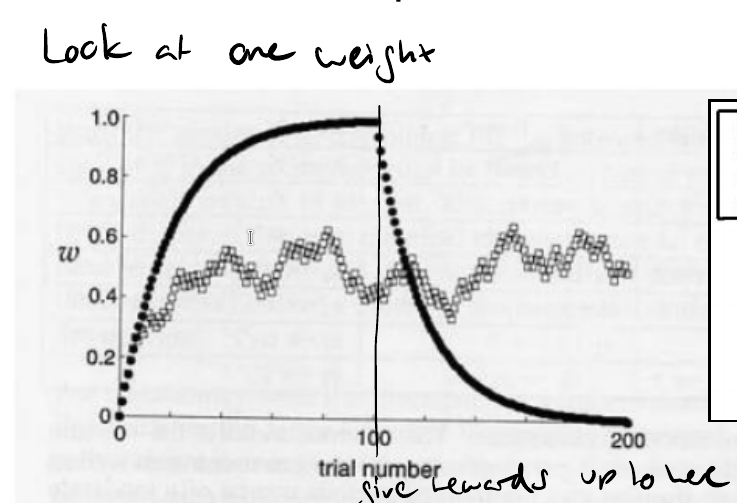
\includegraphics[width=0.9\linewidth]{08_ReinforcementLearning/figures/rw-rule.png}
	\label{fig:rw-rule}
	\caption{Typical exponential / log behavior of the iterative R-W rule.}
\end{figure}


\subsubsection{Temporal Difference Rule to Q-Learning}
The lecture went over these learning rules very quickly and in an unsual order. If you are a beginner, I suggest that you read the sections about MC, MRP and MDP first.

Key Idea of the temporal difference rule (TDR): 
Update the value of the current state based on the immediate reward and the estimated value of the next state. 
Interpretation: we must not look at immediate rewards only but future rewards should be taken into consideration as well on a discounted valuation. 
We assume that the path that our agent takes to navigate the system is given.


\begin{equation}
    V(s_{t}) \leftarrow V(s_t) + \eta[r_{t+1} + \gamma V(s_{t+1}) - V(s_t) ]
\end{equation}

where:

\begin{itemize}
    \item $V(s_t)$: previous estimate
    \item $r_{t+1}$ next reward
    \item $\gamma V(s_{t+1})$ discounted value on the next step
\end{itemize}

Lets now include the fundamental concept of an action to this equation. This adds one dimension to the value function and gives the agent a choice. This new function is called $Q(s,a)$. 

\begin{equation}
Q(s,a) = \mathbb{E}_{(r',s')|s,a}[r+ \gamma  max_{a'}[Q(s',a')]]
\end{equation}
 
By just a few trivial steps one can show that the TD rule is used to get the convex combination in the Q-Learning update rule (different from Q-Function) between old and new $Q$ value seen in the literature:
\begin{align}
Q(s,a)& \leftarrow (1-\alpha_t)Q(s,a) + \alpha_t(r+\gamma max_{a'}[Q(s',a')]) \\
Q(s,a)& \leftarrow Q(s,a) - \alpha_t Q(s,a)  + \alpha_t r + \gamma \alpha_t max_{a'}[Q(s',a')] \\
Q(s,a)& \leftarrow Q(s,a) + \alpha_t (r + \gamma max_{a'}[Q(s',a')] - Q(s,a)) \\
Q(s,a)& \leftarrow Q(s,a) + \alpha_t (r + \gamma max_{a'}[Q(s',a') - Q(s,a)])
\end{align}

Given this rule, we can create and update a map over future states and actions. We can optimize w.r.t the action to get an optimal path (policy). The key idea idea is that we do not need to know any transition probabilities to learn (model), we just need an unbiased estimate from our world (sample). We can get these samples by just playing the "game". If we store the actions $a$ and rewards $r$ from these samples, we can directly apply Q-learning. Thus, Q-learning is considered model-free.

Keep in mind that (in the end), the optimal policy can be deducted from the optimal value function $V^*$:

\begin{equation}
    V^*(x) = max_a Q^*(x,a)
\end{equation}


\subsection{Introduction to Reinforcement Learning}
We saw the concept of looking at expected reward and choosing actions to maximize this reward, but the idea was not well embedded into a generalizing concept. 
Reinforcement learning (RL) exactly puts a name on this framework, which includes Q-Learning as well.
RL is about an agent taking suitable action to maximize reward in a particular situation. 
It is employed by various software and machines to find the best possible behavior or path it should take in a specific situation. 

\begin{figure}[H]
	\centering
	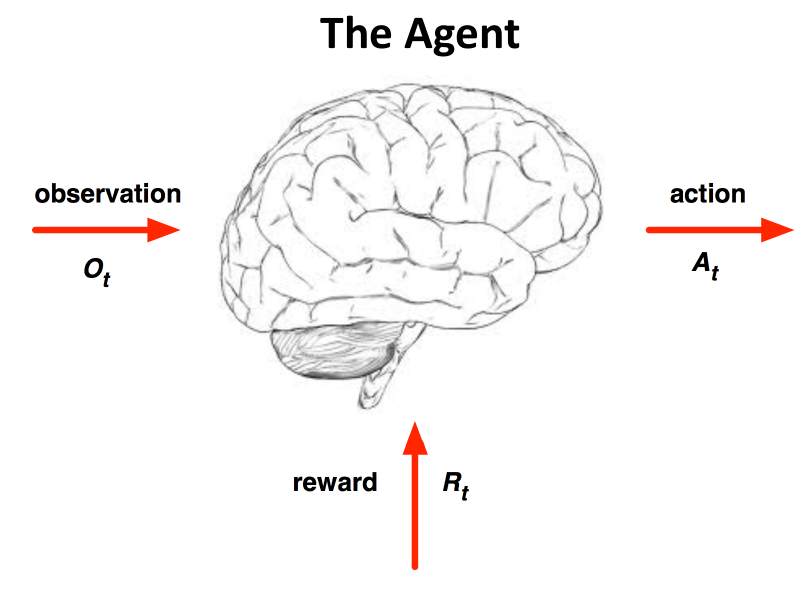
\includegraphics[width=0.9\linewidth]{08_ReinforcementLearning/figures/rl-basic-comps.png}
	\label{fig:rl-basic-comps}
	\caption{Influences from and to the agent in RL to the surrounding world. At each step $t$, the agent exectues an action $A_t$ which the environment recieves. The agent recieves an observation $O_t$ of the environment, for example trough a sensor and the agent is rewarded $R_t$ by its behavior from the environment.}
\end{figure}


Reinforcement learning is based on the reward hypothesis:
\textbf{All goals of an agent can be described by the maximization of expected cumulative reward.}

Example rewards:

\begin{itemize}
    \item Fly stunt maneuvers in an RC helicopter (+ following desired trajectory, - crashing)
    \item Defeat the world champion at Backgammon (+ winning /- loosing)
    \item Manage an investment portfolio (+ more / -  less money)
    \item Make a humanoid robot walk (+ reward for forward motion / − reward for falling over)
    \item Play Atari games better than humans (+/− reward for increasing/decreasing score)
\end{itemize}

The fact that reward presented to the agent is not always immediate leads to the exploration / exploitation dilemma. (Example: A financial investment may take months to mature). 
An agent does not intrinsically know the future implications of its actions, or (how actions interact with) dynamics of the environment.

At each point in time, the agent is in a state. because this information state is all that is necessary to fully determine the agent, it is also said that the state is markovian. This means we can throw away the histrory.

\begin{equation}
    P(S_{t+1}|S_t) = P(S_{t+1} | S_{1:t})
\end{equation}

An RL agent may compute different functions on top of its state.

\subsubsection{Policy}
The agents behavior function callend policy maps from state $s$ to action $a$. The policy may be stochastic or deterministic:

\begin{align}
    a & = \pi(s) \\
    \pi(a|s) & = P(A_t = a | S_t = s)
\end{align}

\subsubsection{Value Function}
Value function is a prediction of future rewards and does so by assigning a number to every state $s$. It depends on a policy $\pi$ to determine where the agent could go and a probability distribution $p(X'|\pi(X), X)$.

We compute this value as expectation over the joint distribution:
\begin{equation}
p(S_{1}, S_{2}, S_{3}, \dots)
\end{equation}

The value function is defined as: 
\begin{equation}
    v_{\pi} = \mathbb{E}[r(s_0, \pi(s_0)) + \gamma r(s_1, \pi(s_1)) + \gamma^2 r(s_2, \pi(s_2)) + \dots]
\end{equation}

But in the  lecture, they mentioned (and it is not distinguished between the two) the conditional value function:

\begin{equation}
    v_{\pi}(s_0) = \mathbb{E}[\sum_{t=0}^\infty \gamma^t r(s_t, \pi(s_t)) | S_0 = s_0]
\end{equation}

Which can be rewritten to the recursive equation (often in the literature):
\begin{equation}
v_{\pi}(s) = r(s_0, \pi(s_0)) + \gamma \sum_{s_1} p(S_1 =s_1 | S_0 = s_0, \pi(s_0)) v_\pi (s_1)
\end{equation}

\subsubsection{Model}
From the previous section we see that we require a probability distribution that depends on direct actions $a$ or a policy returning actions $\pi$:

\begin{align}
    P_{s_t,s_{t+1}} &= p(S_{t+1} = s_{t+1} | S_t = s_t, \pi(s_t)) \\
                    &= p(S_{t+1} = s_{t+1} | S_t = s_t, A_t = a_t)
\end{align}

that predicts the next (immediate) reward:

\begin{equation}
    R_{s_t} = \mathbb{E}[R_{t+1} | S_t = t, A_t = a_t]
\end{equation}

This is called the model. Model free RL uses tricks to not compute / require this distribution. As it is often intractable. Imagine the state space being the  input of a video game!


\begin{figure}[H]
	\centering
	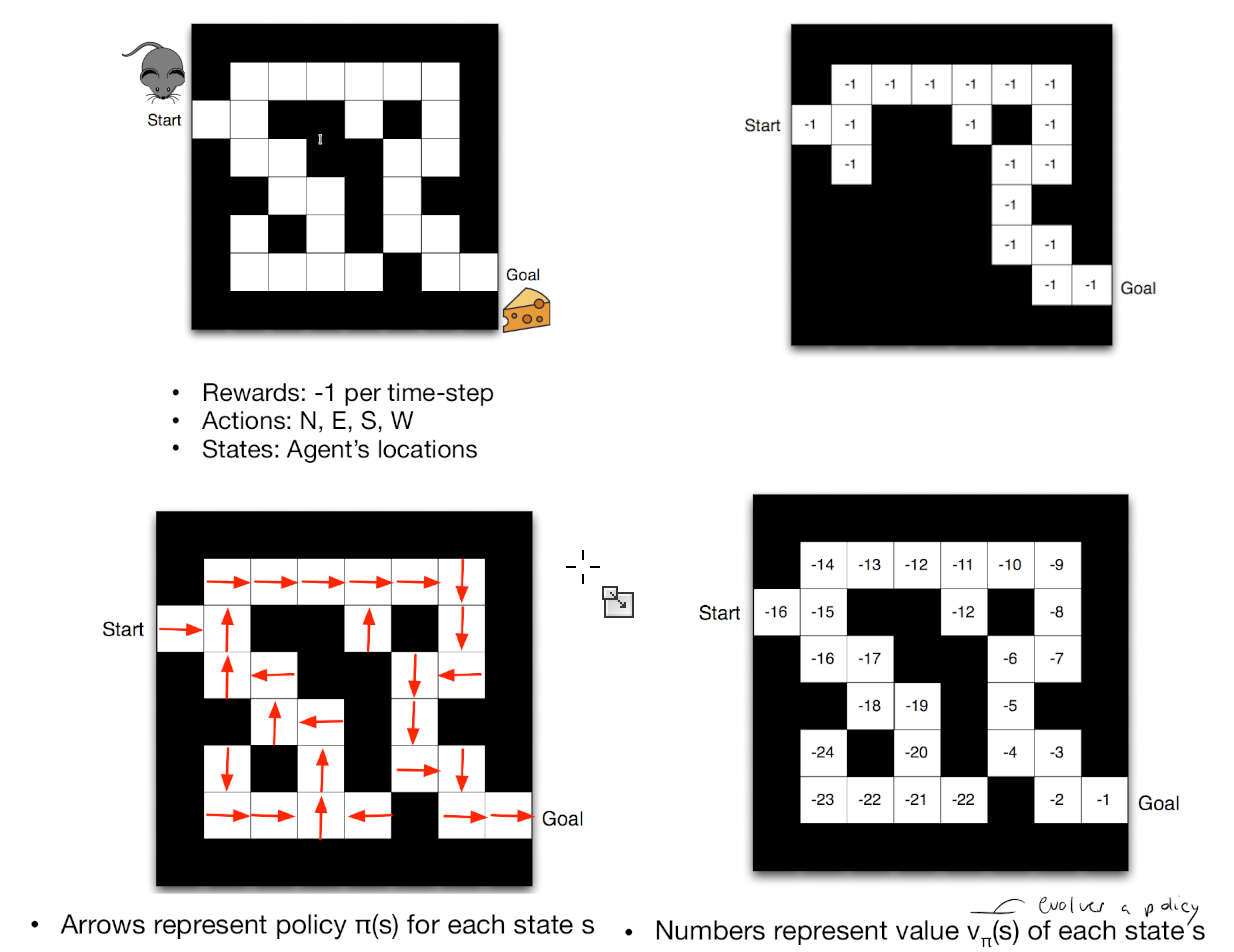
\includegraphics[width=1\linewidth]{08_ReinforcementLearning/figures/rl-example.png}
	\label{fig:rl-example}
	\caption{A small example of a mice showing all the agent related components together with some numbers. (top left) Actions, start, end and definition of other states (the maze). (top right) immediate rewards. (bottom) Policy and value function for each state.}
\end{figure}

Some details to Figure \ref{fig:rl-example}:
\begin{itemize}
    \item Agent may have an internal model of the environment.
    \item Dynamics: How actions change the state.
    \item Rewards: How much reward from each state.
    \item The model may be imperfect.
    \item Grid layout represents transition model $P_{s_t,s_{t+1}}^a$
    \item Numbers (top right) represent immediate reward $R_{s_t}^a$ from each state s.
\end{itemize}

We've seen different RL-subtypes that need to be distinguished. Comment: From the Bellman Theorem we know that every value function induces a policy and every policy induces a value function:

\begin{itemize}
    \item Value Based
       \begin{itemize}
            \item No Policy (Implicitly given by value function, see Bellman Eq.)
            \item Value Function
       \end{itemize}
    \item Policy Based
       \begin{itemize}
            \item Policy
            \item No Value Function (Even tho values can be computed off a policy)
       \end{itemize}
\end{itemize}

Model Free vs model based: We can have a policy and/or a value function in each case, but we distinguish by the need for the model distribution.

\subsubsection{A more sophisiticated Example: Atari}

\begin{figure}[H]
	\centering
	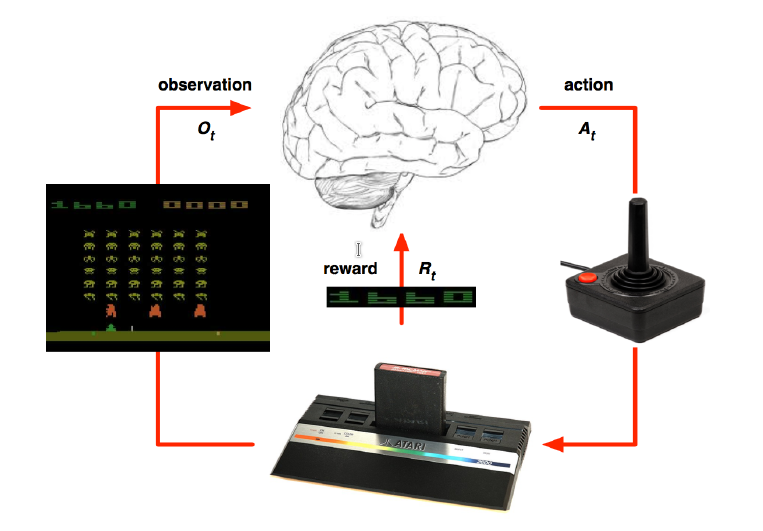
\includegraphics[width=0.9\linewidth]{08_ReinforcementLearning/figures/atari.png}
	\label{fig:rl-atari}
	\caption{The Atari video gaming platform provides and ideal environment to test RL / Planning strategies. For some games, we don't know the rules and apply RL. This means we learn directly from interactive gameplay. Pick actions on a joystick and observe the pixels. For other games we know the rules. This allows to apply planning strategies where we might ask ourselves: What would the next state be? What would the score be?. We can query the future by tree search to some extent.}
\end{figure}

\subsection{Planning}
Even tho planning appears later in the lecture it is actually the logical step before we arrive at RL. It is  a more constrained view where a model of the environment is known. 
The agent performs computations with its model (without any external interaction). 
This is a simplification compared to RL where the environment is initially unknown and the agent may only discover it by interacting with the environment. 
In RL, the agent improves its policy or value function.


If the agent/solver has access to the model, i.e $p(s'|s,a)$ and $r(s,a)$, and it employs it when optimizing the MDP, then we are in the planning settings (or dynamic programming , DP, setting). Otherwise, we are in the RL settings. Of course, sometimes, even though we have access to the model, still we do RL since it is hard to solve directly the MDP, and we prefer to interact with the MDP rather then solving it, i.e., we ignore the model. Remark: I think this is true for most games and therefore, the Atari example might be confusing.


In a planning scenario, we can query the future trough the emulator. We can therfore play / plan ahead to find the optimal policy by tree search. As already mentioned, this might not be possible even for simple games (check out the AlphaGo strategies).

RL on the other hand can be as well refered to as "trial-and-error" learning. However, obviously we try to guide the agent to loose the least amount of reward that is possible.

\subsection{Exploration / Exploitation}
Everyone is confronted with the same dilemma on a daily basis: should I keep doing what I do, or should I try something else.
For example should I go to my preferred restaurant or should I try a new one, should I keep my current job or should I find a new one, etc…

In Reinforcement Learning, this type of decision is called exploitation when you keep doing what you were doing, and exploration when you try something new.

\begin{itemize}
    \item Exploration finds more information about the environment. 
    \item Exploitation exploits known information to maximize reward. It is usually important to explore as well as exploit
\end{itemize}


\subsection{Basics}
Remark: In my opinion these chapters build the foundation for RL but in the lecture they appear after RL and thus I kept that order.
If you are a beginner to these topics, 
I highly recommend to gain some basic knowledge about probabilistic graphical models (PGM) (Bayesian networks) first. 
They are used from here on, but were not introduced explicitly in the lecture.

\subsubsection{Markov Chain (MC)}
A Bayesian network is a kind of PGM that uses a directed (acyclic) graph to represent a factorized probability distribution and associated conditional independence over a set of variables. 
Definition: A state $S_t$ is Markov if and only if:

\begin{equation}
    P(S_{t+1}|S_t) = P(S_{t+1} | S_{1:t})
\end{equation}

where $s_t$ is the current state and $s_{t+1}$ is the successor state.

The state captures all relevant information from the history. 
Once the state is known, the history may be thrown away. This means that the state is a sufficient statistic of the future.

The state transition matrix $P$ defines transition probabilities from all states $m = s_t$ to all successor states $n = s_{t+1}$. :

\begin{equation*}
P_{m,n} = 
\begin{pmatrix}
P_{1,1} & P_{1,2} & \cdots & P_{1,n} \\
P_{2,1} & P_{2,2} & \cdots & P_{2,n} \\
\vdots  & \vdots  & \ddots & \vdots  \\
P_{m,1} & P_{m,2} & \cdots & P_{m,n} 
\end{pmatrix}
\end{equation*}

\begin{figure}[H]
	\centering
	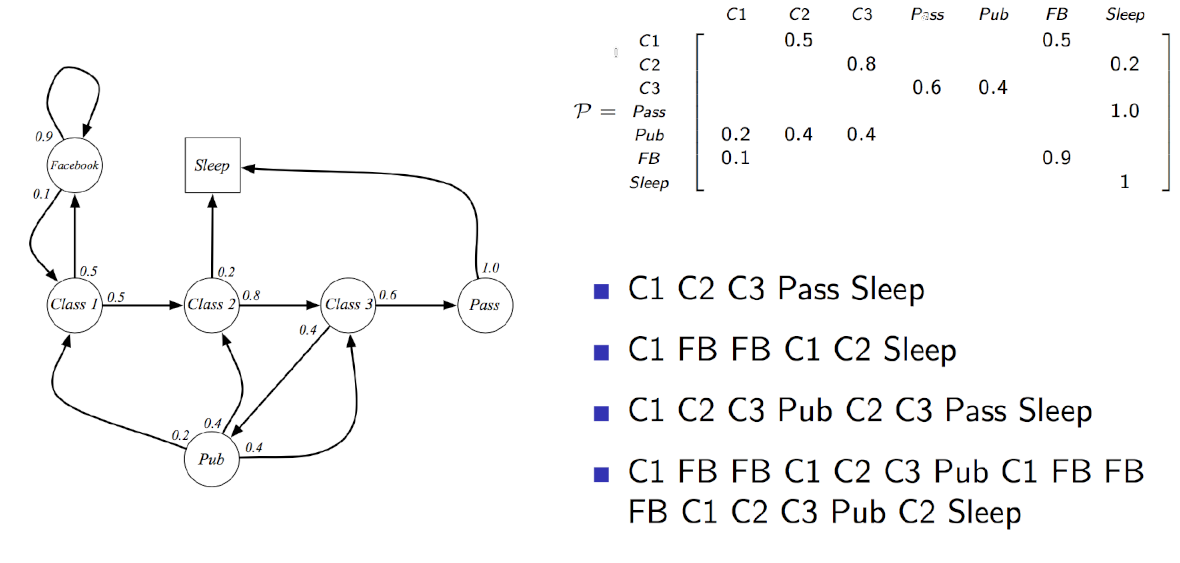
\includegraphics[width=0.9\linewidth]{08_ReinforcementLearning/figures/mc-student-ex.png}
	\label{fig:mc-student-ex}
	\caption{(left) An example Markov chain showing all state transition probabilites next to its nodes. (right) The corresponding state transition matrix and results of a sampling procedure applied to this Markov chain. Be aware that this is not a PGM, the nodes are not random variables.}
\end{figure}


\subsubsection{Markov Reward Process (MRP)}
A Markov reward process is a stochastic process which extends either a Markov chainby adding a reward rate to each state.

Definition: A Markov Reward Process is a tuple $(S, P, R, \gamma) $ where 
$S$ is a finite set of states, 
$P$ is a state transition probability matrix $P_{t,t+1} = P(S_{t+1}|S_t)$,
$R = \mathbb{E}[R_{t+1}|S_t=s]$ is a reward function and
$\gamma$ is a discount in the interval $(0,1)$

Facts:
\begin{itemize}
    \item Mathematically convenient to discount rewards. It avoids infinite returns in cyclic Markov processes.
    \item Uncertainty about the future may not be fully represented.
    \item If the reward is financial, immediate rewards may earn more interest than delayed rewards.
    \item Animal/human behavior shows preference for immediate rewards.
    \item It is sometimes possible to use un-discounted Markov reward processes (i.e. $\gamma$ = 1), e.g. if all sequences terminate.
\end{itemize}

We call $G_t$ the return which is the total discounted reward from time step $t$ onward.

\begin{equation}
    G_t = \sum_{k=0}^\infty \gamma^k R_{t+k+1}
\end{equation}

If we just look at $G_t$ we must assume that we know the chain of events that lead to the specific rewards $R$, 
however the MRP is a stochastic process. 
Therefore we may compute the conditional value function given that we know where we start ($s_t$).
We've seen this function before in the RL chapter:

\begin{equation}
    v_{s_t} = \mathbb{E}[R_{t+1} + \gamma R_{t+2} + \gamma^2 R_{t+3} + \dots| S_t = s_t]
\end{equation}

which is just

\begin{equation}
    v_{s_t} = \mathbb{E}[G_t|S_t = s_t]
\end{equation}


\begin{figure}[H]
	\centering
	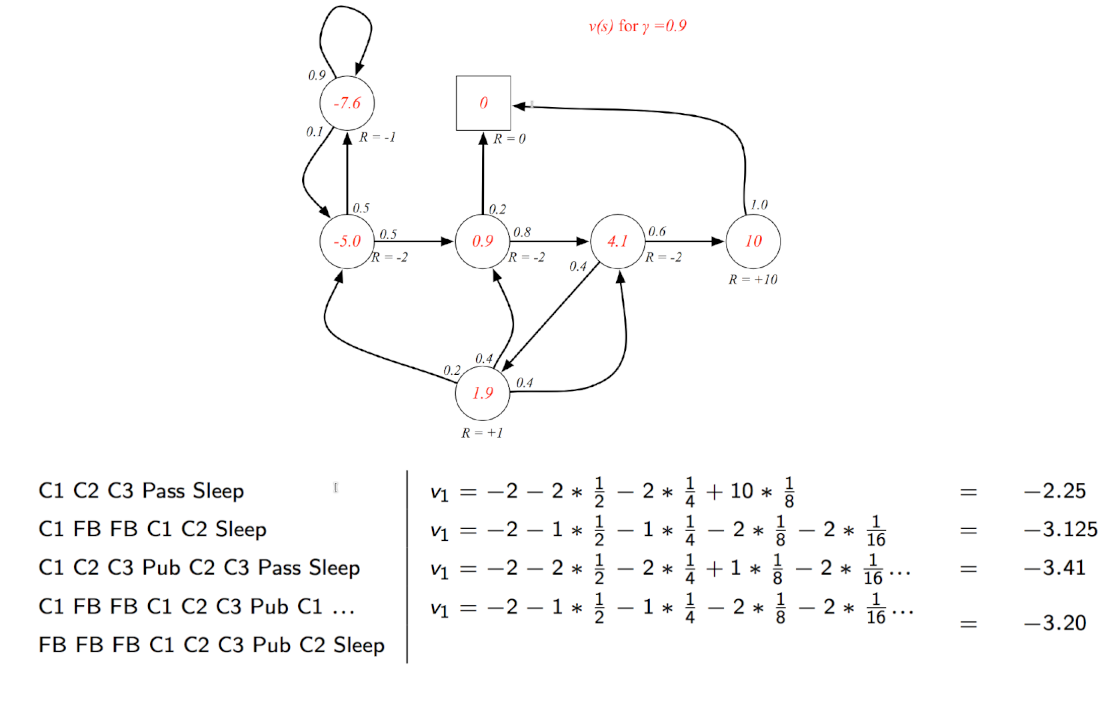
\includegraphics[width=0.9\linewidth]{08_ReinforcementLearning/figures/mrp-example.png}
	\label{fig:mrp-example}
	\caption{The MC of \ref{fig:mrp-example} extended to be a MRP. We may compute the random samples return.}
\end{figure}



\subsubsection{Markov Decision Process (MDP)}
Markov decision process (MDP) is a Markov reward process with decisions (actions that we can take). It is still an environment in which all states are Markov.
Definition: A Markov Reward Process is a tuple $(S, A, P, R, \gamma) $ where
$S$ is a finite set of states, 
$A$ is a finite set of actions, 
$P$ is a state transition probability matrix $P_{t,t+1} = P(S_{t+1}|S_t, A_t)$,
$R = \mathbb{E}[R_{t+1}|S_t=s, A_t=a]$ is a reward function and
$\gamma$ is a discount in the interval $(0,1)$

Markov decision processes formally describe an environment for reinforcement learning where the environment is fully observable.
Almost all RL problems can be formalized as MDPs:

\begin{itemize}
    \item Partially observable problems can be converted into MDPs.
    \item One Armed Bandits are MDPs with one state.
\end{itemize}

\begin{figure}[H]
	\centering
	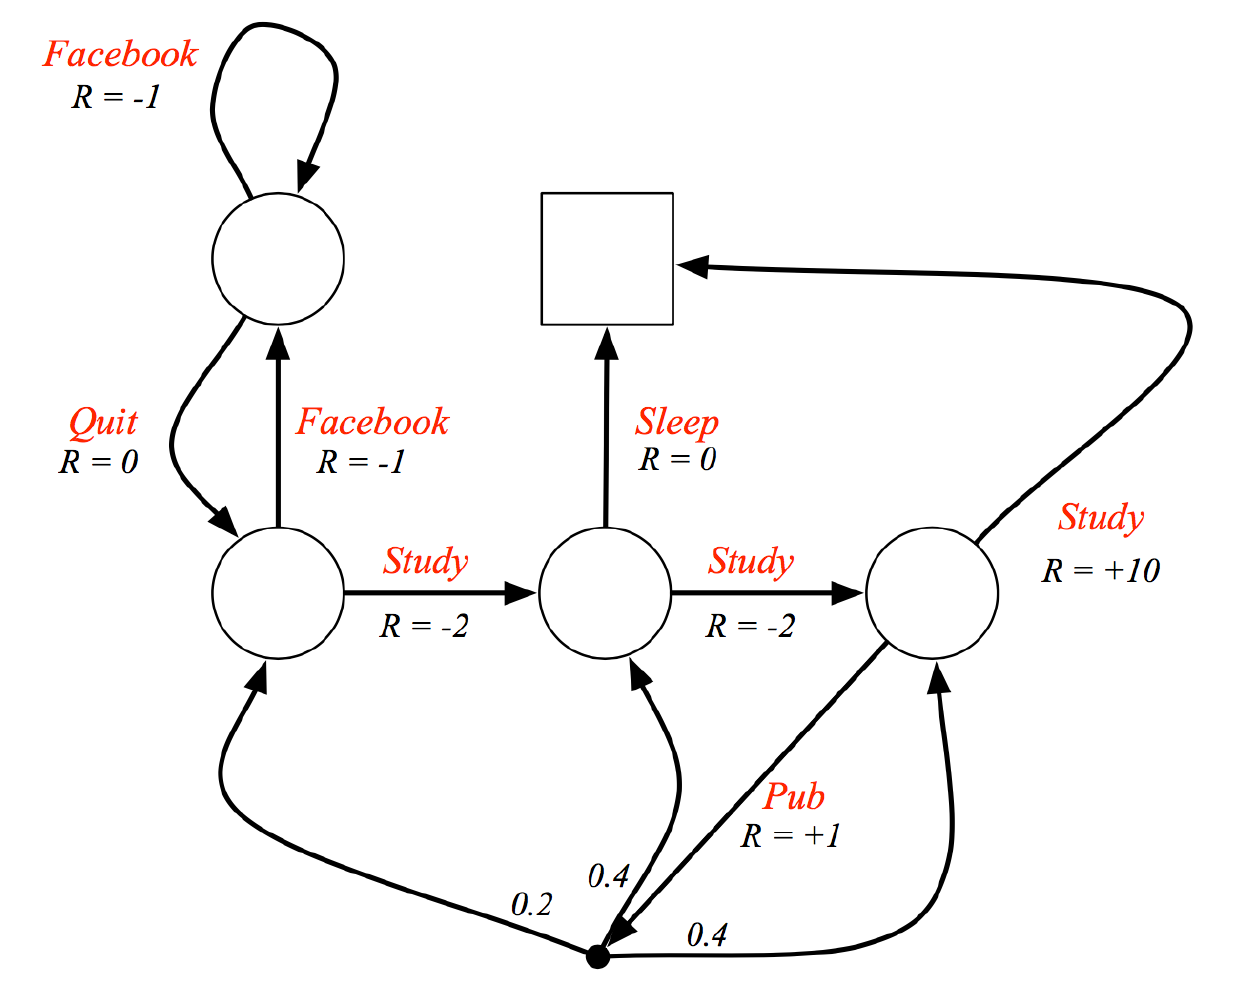
\includegraphics[width=0.9\linewidth]{08_ReinforcementLearning/figures/mdp-example.png}
	\label{fig:mrp-example}
	\caption{The MC of \ref{fig:mrp-example} extended to be a MRP extended again to be an MDP. However we should be careful with the comparisons. In the MRP, our agent was guided purely by randomness and we had no choice. Now, the agent is able to directly influence its path. Note that some of the transitions are deterministic. For example if we quit facebook, we are for sure back to studying, however if were in the pup, we might be too drunk and randomness influences the outcome.}
\end{figure}

One can see that we are very close now to what we introduced in the RL section, however one key piece is missing.  Given that we have choice as an agent now, how do we know the optimal behavior?

\subsubsection{Bellman Equation}
The Bellman equation (BE), named after Richard E. Bellman, is a necessary condition for optimality associated with the mathematical optimization method known as dynamic programming (aka. RL where the environment is known $\longrightarrow$ MDP). It allows us to "solve" the MDP problem, the problem of not knowing how to act in an environment where we are able to take action.


\textbf{BE in MRP}
In the most simple case, we can just evaluate the Bellman expectation equation in an MRP where we have no policy to optimize.

\begin{align}
    v_{s_t} &= \mathbb{E}[G_t|S_t = s_t] \\
    & = \mathbb{E}[R_{s_{t+1}} + \gamma R_{s_{t+2}} + \gamma^2 R_{s_{t+3}} + \dots| S_t = s_t] \\
    & = \mathbb{E}[R_{s_{t+1}} + \gamma (R_{s_{t+2}} + \gamma R_{s_{t+3}} + \dots)| S_t = s_t] \\
    & = \mathbb{E}[R_{s_{t+1}} + \gamma (G_{t+1})| S_t = s_t] \\
    & = \mathbb{E}[R_{s_{t+1}} + \gamma v(S_{t+1})| S_t = s_t] \\
\end{align}

This is the immediate reward $R_{t+1}$ plus the discounted value of the successor state $\gamma v(S_{t+1})$.
This is again close to the temporal difference rule. 
If we move the reward from the next state to the current one (by definition), we can pull $R_{s_t}$ out of it and compute the expected value trough the sum and the equation becomes:

\begin{equation}
   v_{s_t} = R_{s_t} + \gamma \sum_{s_{t+1} \in S} P_{s_t,s_{t+1}} v(s_{t+1})
\end{equation}

\begin{figure}[H]
	\centering
	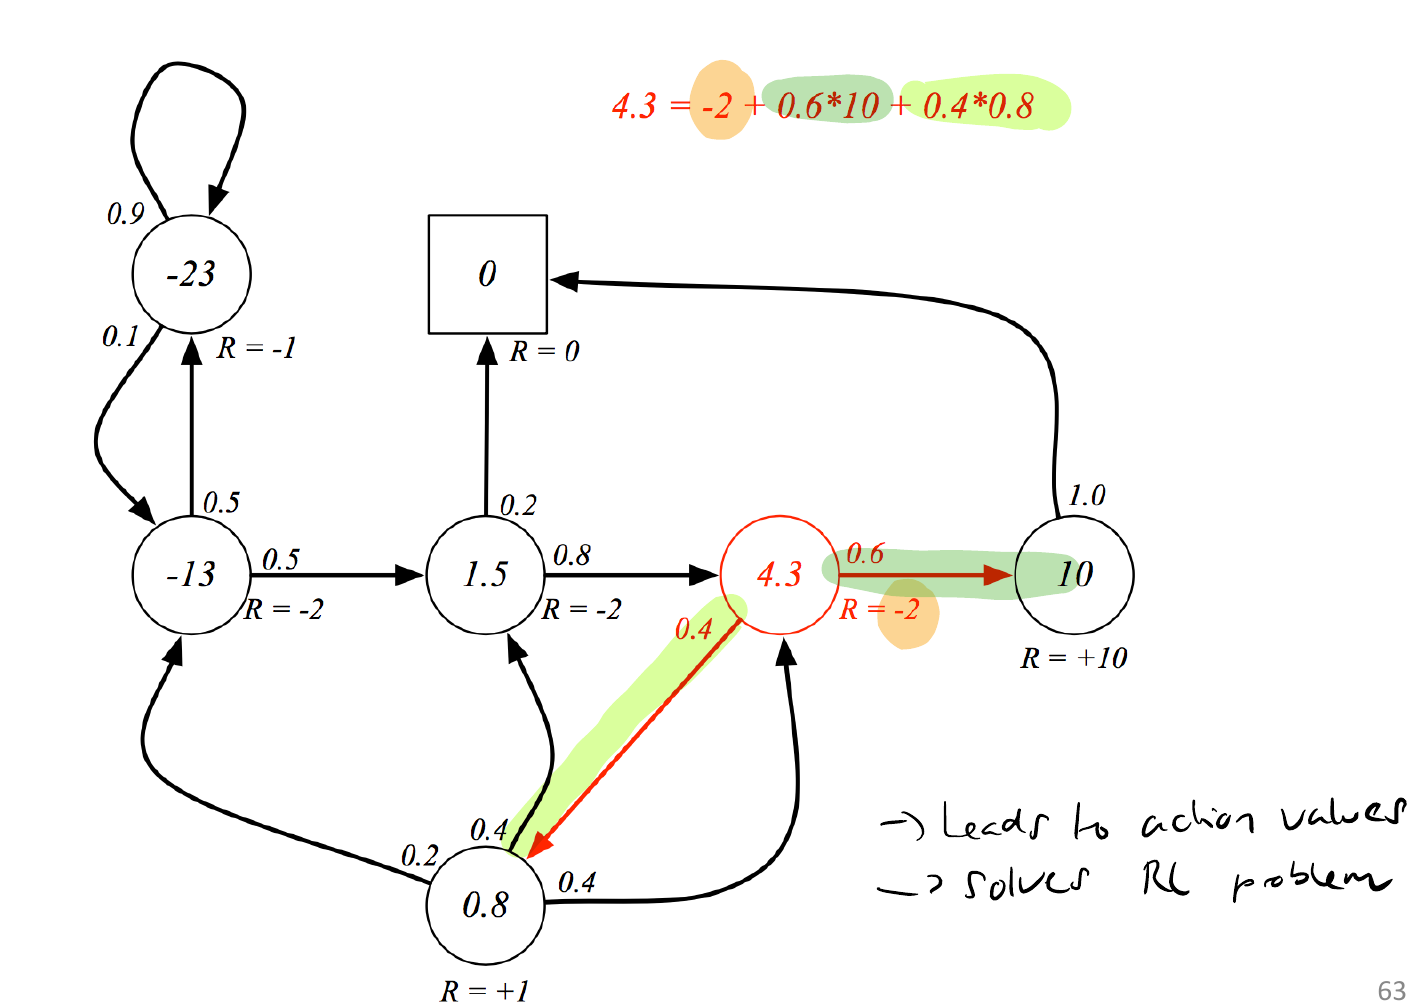
\includegraphics[width=0.9\linewidth]{08_ReinforcementLearning/figures/bellmann-mrp.png}
	\label{fig:mrp-example}
	\caption{Example computation of the value of the red node in an MRP.}
\end{figure}

One might argue that this leads to action values by choosing the next state based on its value "score". Also this can be solved explicitly as a linear system.


\textbf{BE in MDP}
In MDP, we must somehow include the actions. Over the entire task, the actions we take are defined to be the policy. Since we can optimize this policy, one might ask how to do this using the Bellman optimality equation.

\begin{itemize}
    \item The state-value function $v_\pi(s)$ of an MDP is the expected return starting from state $s$, and then following policy $\pi$.
    \item The action-value function $q_\pi(s,a)$ is the expected return starting from state $s$, taking action $a$, and then following policy π.
\end{itemize}

We may rewrite both in a similar maner as we did in the MRP case.
\begin{align}
    v_\pi(s_t) &= \mathbb{E}_\pi[G_t|S_t = s_t] \\
    &= \mathbb{E}_\pi[R_{s_{t+1}} + \gamma v_\pi(S_{t+1})|S_t = s_t] \\
\end{align}

And if we again shift the reward ($\overset{!}{=}$):
\begin{align}
    q_\pi(s_t,a_t)& = \mathbb{E}_\pi[G_t|S_t = s_t, A_t =a_t] \\
    &= \mathbb{E}_\pi[R_{s_{t+1}} + \gamma q_\pi(S_{t+1}, A_{t+1})|S_t = s, A_t=a] \\
    & \overset{!}{=} R_{s_t}^{a_t} + \gamma \sum_{s_{t+1} \in S} P_{s_t,s_{t+1}}^{a_t} v(s_{t+1}) \\
    & = R_{s_t}^{a_t} + \gamma \sum_{s_{t+1} \in S} P_{s_t,s_{t+1}}^{a_t} \sum_{a_{t+1} \in A} \pi(a_{t+1}|s_{t+1}) q_\pi(s_{t+1}, a_{t+1})
\end{align}

As you can see, the notation becomes quite tedious. From now on we use $S_t = s$ and $S_{t+1} = s'$. The same applies to actions.

\begin{figure}[H]
	\centering
	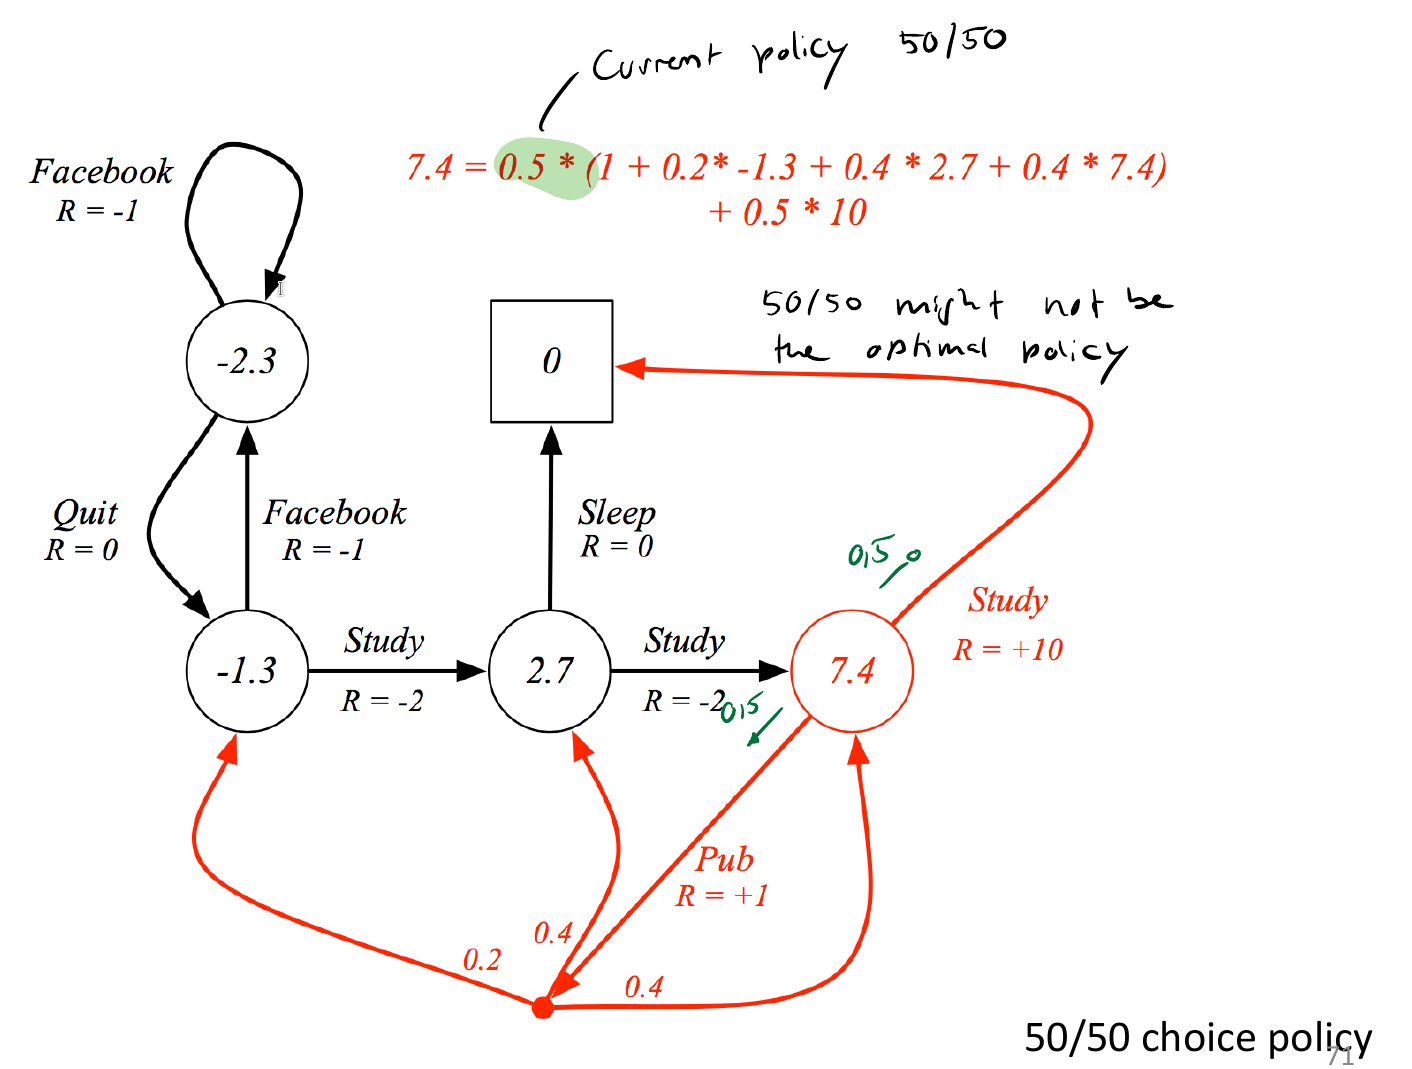
\includegraphics[width=0.9\linewidth]{08_ReinforcementLearning/figures/bellmann-mdp.png}
	\label{fig:mrp-example}
	\caption{Example of policy based computation of the value of the red node in an MDP.}
\end{figure}

\textbf{Finding the optimal action-value (Q) function}

We can now define the optimal value function:
\begin{equation}
    v^*(s) = max (v_\pi(s))
\end{equation}

and the optimal action-value (q) function:

\begin{equation}
    q^*(s,a) = max (q_\pi(s,a))
\end{equation}

You may noticed that we depend on the policy for  $v^*(s)$ and $q^*(s,a)$.
An optimal policy can be found by maximizing over the optimal Q-function $q^*(s,a)$:

\begin{equation*}

\pi^*(a|s) =     
\begin{cases}
    1, & \text{if } a = argmax_{a \in A}(q^*(s,a)) \\
    0, & \text{otherwise}
\end{cases}
    
\end{equation*}


There is always a deterministic optimal policy for any MDP.
If we know $q^*(s,a)$, we immediately have the optimal policy.

In the last step, this theorem allows us to assemble the Bellman optimality update equations:

We now use the optimal value function ($v^*(s) = max (v_\pi(s))$) to get the optimal Q-function:

\begin{equation}
        q^*_\pi(s,a)& = R_t^a + \gamma \sum_{s' \in S} P_{s,s'}^a v^*(s') \\ 
\end{equation}

Note that the agent has to average, because we can't choose. This is decided by the environment.
Finally we may write down the Bellman optimality equations for $v^*$ and $q^*$:


\begin{equation}
    v^*(s) \leftarrow max_a [R_{s}^a + \gamma \sum_{s' \in S} P_{s,s'}^a v^*(s')]
\end{equation}

\begin{equation}
    q^*(s, a) \leftarrow R_{s}^a + \gamma \sum_{s' \in S} P_{s,s'}^a max_{a'} [q^*(s', a')]
\end{equation}

Bellman figured out that our policy being optimal means that we can be greedy w.r.t these optimality equations.
If we update over and over again, we will converge to a fixed point which is the optimal policy.



\subsection{Deep Reinforcement Learning}
In the previous sections, distributions were always treated as discrete tables. This is not possible for large state/action spaces. Therefore, functional approximations to these functions must be found. We've already seen that deep neural networks (DNN) are function approximators in their nature. One can parametrize a policy or Q-function and use DNN to estimate its parameters directly from state space.

For optimization purposes, we define a loss function. This loss follows from moving Q inside of expectation.

\begin{equation}
    L = \frac{1}{2}[r + max_{a'}Q(s',a') - Q(s,a)]^2 
\end{equation}

We find the optimal action-value function $Q^*$ by parametrizing it with $\theta$ (make it DNN compatible).

\begin{equation}
    Q^*(s,a) =  max_\pi \mathbb{E}[r_t + \gamma r_{t+1} + \gamma^2 r_{t+2} + \dots | s_t =  s, a_t = a, \pi]
\end{equation}

and then minimize the loss w.r.t $\theta$. Comment: Often, we approximate $\mathbb{E}$ by sampling.

\begin{equation}
    L_i(\theta_i) = \mathbb{E}_{s,a,r,s'~U(D)} [r+ \gamma max_{a'}Q(s',a'|\theta_i^-) - Q(s,a|\theta_i)]
\end{equation}

This is again the temporal difference rule.

\begin{figure}[H]
	\centering
	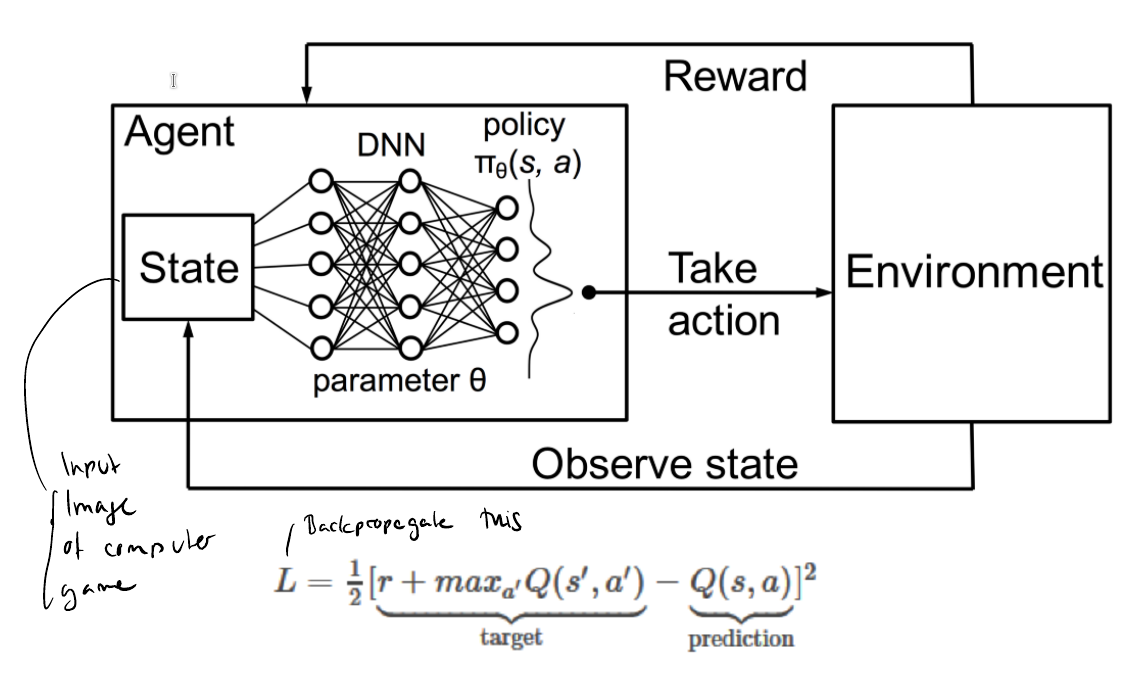
\includegraphics[width=0.9\linewidth]{08_ReinforcementLearning/figures/deep-rl-1.png}
	\label{fig:rl-basic-comps}
	\caption{Main building blocks of a deep RL system.}
\end{figure}

\begin{figure}[H]
	\centering
	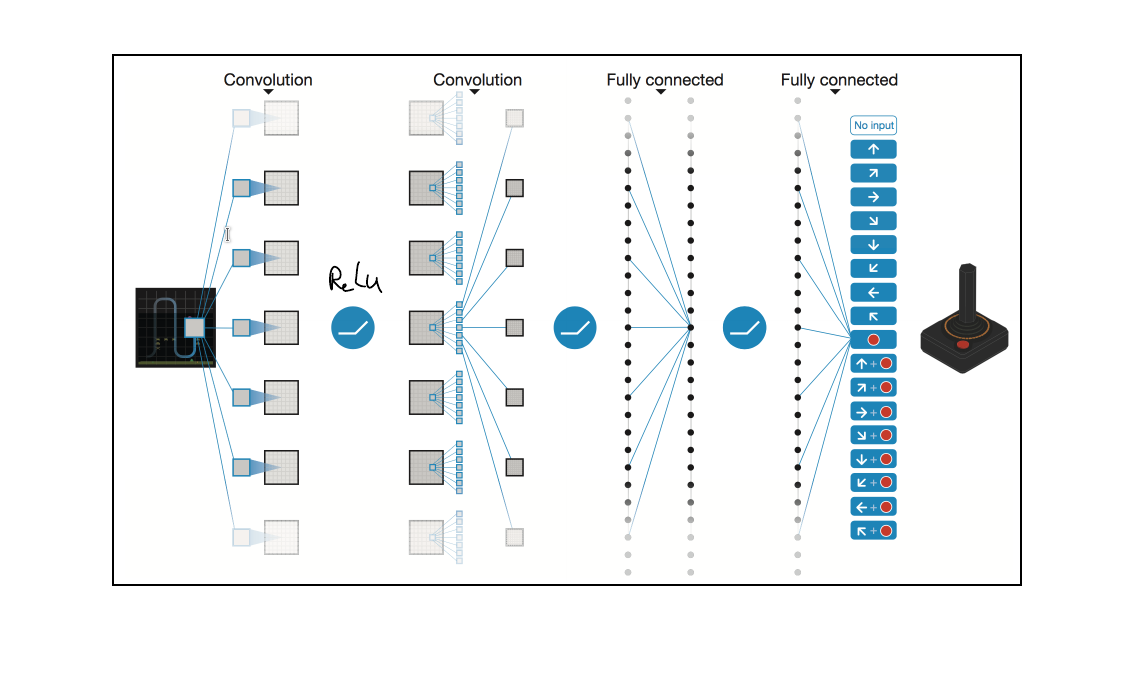
\includegraphics[width=0.9\linewidth]{08_ReinforcementLearning/figures/deep-rl-example.png}
	\label{fig:deep-rl-example}
	\caption{A deep RL system trained directly from input (Atari game video output) to actions of the controlling joystick.}
\end{figure}




\end{document}